\documentclass[
    a4paper
]{scrreprt}
\usepackage[ngerman]{babel}
\usepackage[utf8]{inputenc}
\usepackage{textcomp, expdlist, array, colortbl, xcolor}
\usepackage[pdftex]{graphicx}
\usepackage[TS1, T1]{fontenc}
\usepackage{palatino} % Schriftart
\usepackage{parskip} %Erste Zeile eines Paragrafen nicht einrücken

\usepackage{listings}
\usepackage{color}
\usepackage{xcolor}

% Snippets settings
\lstset{language=C++,
	basicstyle=\ttfamily,
	keywordstyle=\color{blue}\ttfamily,
	stringstyle=\color{red}\ttfamily,
	commentstyle=\color{green}\ttfamily,
	morecomment=[l][\color{magenta}]{\#}
}


\begin{document}
    \sffamily % Whole document sans-serif


    % Titelseite
    \begin{titlepage}
        \centering
        
\includegraphics[width=0.8\textwidth]{./images/logo_hska.png}\par\vspace{1cm}
        \vspace{1cm}

        {\scshape\Large Systemnahes Programmieren\par}
        \vspace{1.5cm}

        {\huge\textbf{Compiler}\par}
        \vspace{2cm}

        {\Large\itshape Timo Blust, 48594\par}
        {\Large\itshape Gennadi Eirich, 50629\par}
        {\Large\itshape Tim Essig, 49683\par}

        \vfill

        % Bottom of the page
        {\large \today\par}
    \end{titlepage}


    % Inhaltsverzeichnis
    \tableofcontents

    % Scanner
    \chapter{Scanner}
    \section{Buffer}
    Die Aufgabe der \textit{Buffer}s besteht darin, die Eingabedatei zu puffern.\\
    
    Für die Realisierung der Aufgabe legt der \textit{Buffer} zwei \textbf{char*} an, mir jeweils der Größe von 2048 (\textbf{HSKA\_BUFFER\_SIZE}). 
    Diese werden mit \textbf{posix\_memalign} allokiert und mit \textbf{memset()} auf \textbf{0} gesetzt. Durch das auf \textbf{0} setzen, kann der \textit{Automat} das Ende der Datei erkennen. Folgender code wird für jedes der zwei Buffer (\textbf{\_previousBuffer, \_currentBuffer}) beim instanziieren aufgerufen.
	    \begin{lstlisting}
int err = posix_memalign(reinterpret_cast<void**>(buffer), 
			 HSKA_BUFFER_SIZE, HSKA_BUFFER_SIZE);
memset(*buffer, 0, HSKA_BUFFER_SIZE); // Fill buffer
		\end{lstlisting}
	
	Um das aktuelle Zeichen vom \textit{Buffer} zu bekommen, wird die Methode \textbf{nextChar()} bereitgestellt. Bei jedem Aufruf von \textbf{nextChar()} wird das aktuelle Zeichen aus dem \textit{Buffer} gelesen und einige der folgenden Offsets werden manipuliert.
	\begin{description}
		\item[\_positionOffset] Das absolute Offset des aktuellen Zeichen (wird bei jedem abgefragten Zeichen inkrementiert)
		\item[\_currentColumnNum] Die aktuelle Spalte des Zeichens. Bei einem Zeilenumbruch wird dieses wieder auf \textbf{1} gesetzt.
		\item[\_filePositionOffset] Offset der Datei. Beim einlesen eines neuen Teils der Datei wird dieser um die Größe des eingelesenen buffers erhöht. 
	\end{description}
	
	Ist \textbf{\_positionOffset} gleich \textbf{\_filePositionOffset}, so ist das Ende des aktuellen \textit{Buffer}s erreicht und es muss ein neues Teil der Eingabedatei mit der Länge \textbf{HSKA\_BUFFER\_SIZE} eingelesen werden.
	\begin{lstlisting}
ssize_t size = read(_fileHandle, _currentBuffer, 
		    HSKA_BUFFER_SIZE);
	\end{lstlisting}
	
	\begin{center}
		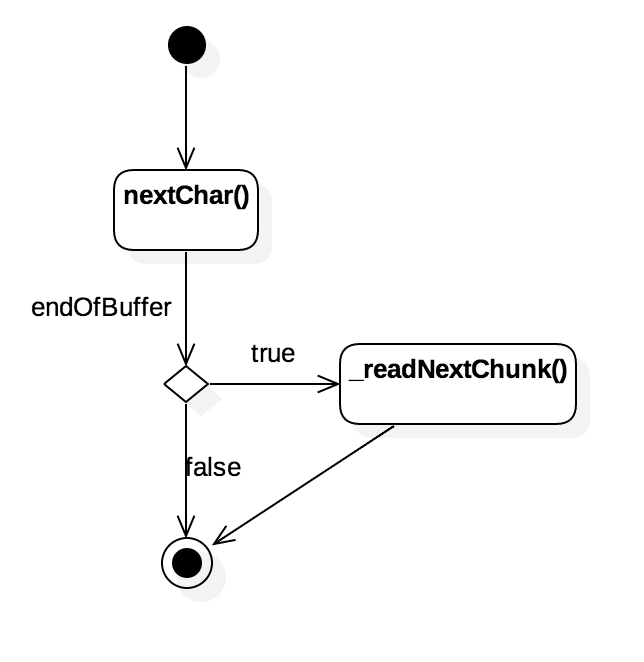
\includegraphics[width=0.5\textwidth]{./images/buffer_activity.png}
	\end{center}
	
	Um die Lexeme und Zahlen bestimmen zu können wird ein kompletter \textit{String} benötigt. Dafür stellt der \textit{Buffer} die Methode \textbf{subString()} bereit. Dieser werden Länge und Offset des geforderten \textit{String}s übergeben.
	Ist der geforderte \textit{String} länger als der Offset (relative Position des letzten Zeichen) des \textbf{\_currentBuffer}, so wird auch aus dem \textbf{\_previousBuffer} gelesen.
    
    
    \section{Symboltabelle}
    
    
    \section{Automat}
    
    
    \section{Scanner}
    Die Aufgabe des \textit{Scanner}s ist dem Aufrufer das nächste \textit{Token} der Eingabedatei zu übergeben und dieses unter Umständen in die \textit{Symboltabelle} einzutragen.\\
    
    Beim Aufruf von \textbf{nextToken()} hold der \textit{Scanner} das nächste Zeichen vom \textit{Buffer} und übergibt es dem Automaten. Wird dabei ein \textit{Token} erkannt, so gibt die Methode des \textit{Automaten} \textbf{true} zurück.

	Wird ein \textbf{IDENTIFIER} erkannt so wieder dessen \textit{String} bestimmt und dieser wird in die \textit{Symboltabelle} eingetragen. Diese, vom Aufruf zurückgegebene \textit{Information}, wird dem \textit{Token} angehängt.
	
	Im Falle eines \textbf{INTEGER} wird ebenso dessen \textit{String} bestimmt und der Wert der Zahl mit \textbf{strtol} bestimmt. Dabei wird überprüft ob die Zahl im Zahlenbereich liegt. Falls nicht, wird ein Fehler auf \textbf{stderr} ausgegeben.
	
	Bei einem gefunden \textbf{ERROR} wird dieses auf \textbf{stderr} ausgegeben mit Zeile, Spalte und dem Symbol.
	
	Alle anderen \textit{Token} werden direkt dem Aufrufer zurückgegeben. 
	
	Des weiteren enthält jedes \textit{Token} die Informationen Typ, Zeile und Spalte.
	
	\begin{center}
		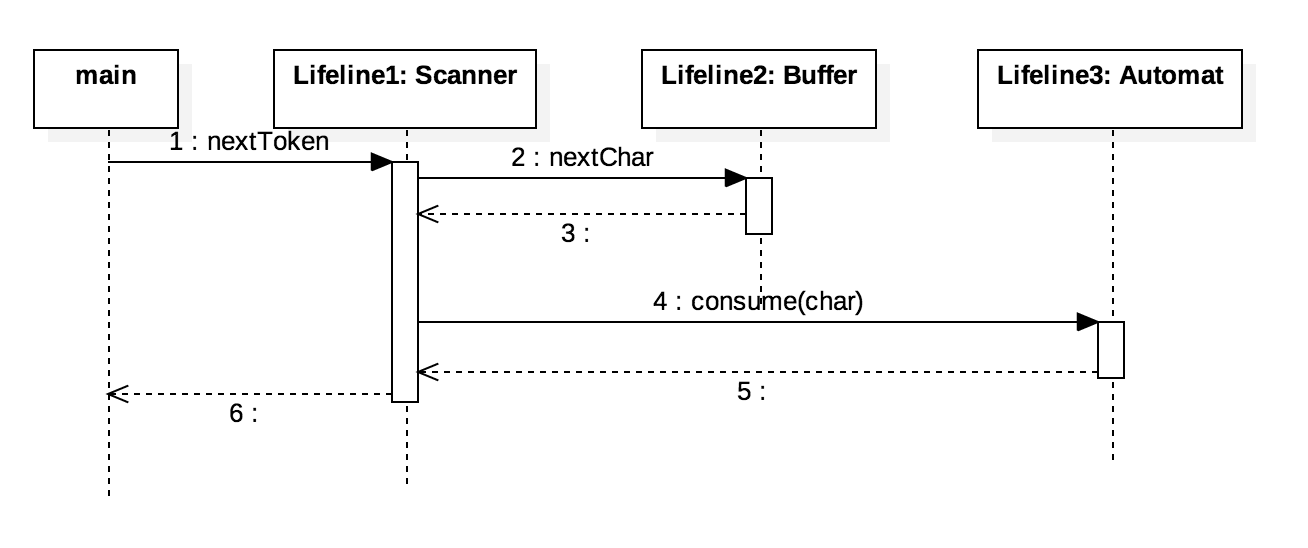
\includegraphics[width=0.8\textwidth]{./images/scanner_sequence.png}
	\end{center}

	Unter gewissen Umständen kann es auch passieren, dass der \textit{Automat} mehrere \textit{Token}s zurückgibt. Dabei wird überprüft ob weitere \textit{Token} an diesem anhängen. Falls dem so ist werden diese lokal abgelegt und beim nächsten Aufruf von \textbf{nextToken()} priorisiert abgearbeitet.
	
	Folgend der Code für das Überprüfen, ob weitere \textit{Token} dem aktuellen anhängen. Da das \textbf{NEW\_LINE}-Token ignoriert wird, wird dieses gelöscht und es wird weiter geprüft. Sollte das nächste ein \textbf{nullptr} sein, so ist das Ende der Liste erreicht und es gibt keine weiteren \textit{Token} mehr. Ab jetzt kann wieder ein Zeichen aus dem \textit{Buffer} eingelesen werden.
    
   	\begin{lstlisting}
void Scanner::_checkForPendingToken(TokenPosition* tokens)
{
 auto next = tokens->getNext();
 if (next == nullptr)
 {
  _pendingTokens = nullptr;
  return;
 }

 // Ignore the NEW_LINE token
 if (next->token == Token::TokenType::NEW_LINE)
 {
  _checkForPendingToken(next); // Check next one for pending token
  delete next; // delete it because its never used/ignored
 }
 else
  _pendingTokens = next;
}
    \end{lstlisting}


	\section{Ausführung}
	Für die Ausführung müssen dem Programm zwei Parameter übergeben werden.

		\begin{enumerate}
			\item Eingabedatei (Sourcecode)
			\item Ausgabedatei (Aufistung aller gefundenen \textit{Token}s)
		\end{enumerate}

	Gebaut wird das Programm mit \textbf{Makefile}.
	
	Folgend die Kommandos für den Bau und die Ausführung des Scanners.
	
	\begin{lstlisting}
$ make 			// im root Ordner
$ cd bin/		// Ordner in dem das target liegt
$ ./HsKA-Scanner eingabedatei.txt ausgabedatei.txt
	\end{lstlisting}
            
	 % Parser
%	\chapter{Parser}

\end{document}
